\section{Image classification}

Image classification involves assigning an input image $\mathbf{I}\in\mathbb{R}^{R\times C \times 3}$ to a label $y$ from a predefined set of categories $\lambda$. 
A classifier is a function $f_\theta$ that maps the image to a label, expressed as:
\[f_\theta:\mathbf{I} \rightarrow f_\theta(\mathbf{I})\in\lambda\]

\subsection{Linear classifier}
To input an image into a neural network, the image is first flattened into a vector, with the RGB color channels linearized column by column.
Each element in this vector corresponds to a neuron in a single-layer neural network, where the number of output neurons matches the number of classification labels.
Each input neuron is fully connected to all output neurons, leading to an impractically large number of connections as image dimensions increase. 
This problem, known as the curse of dimensionality, prevents the straightforward application of deep neural networks to large datasets.

For instance, consider an RGB dataset with $32 \times 32$ images and 6000 examples distributed across ten classes (e.g., CIFAR-10). 
The neural network for this dataset can be visualized as:
\begin{figure}[H]
    \centering
    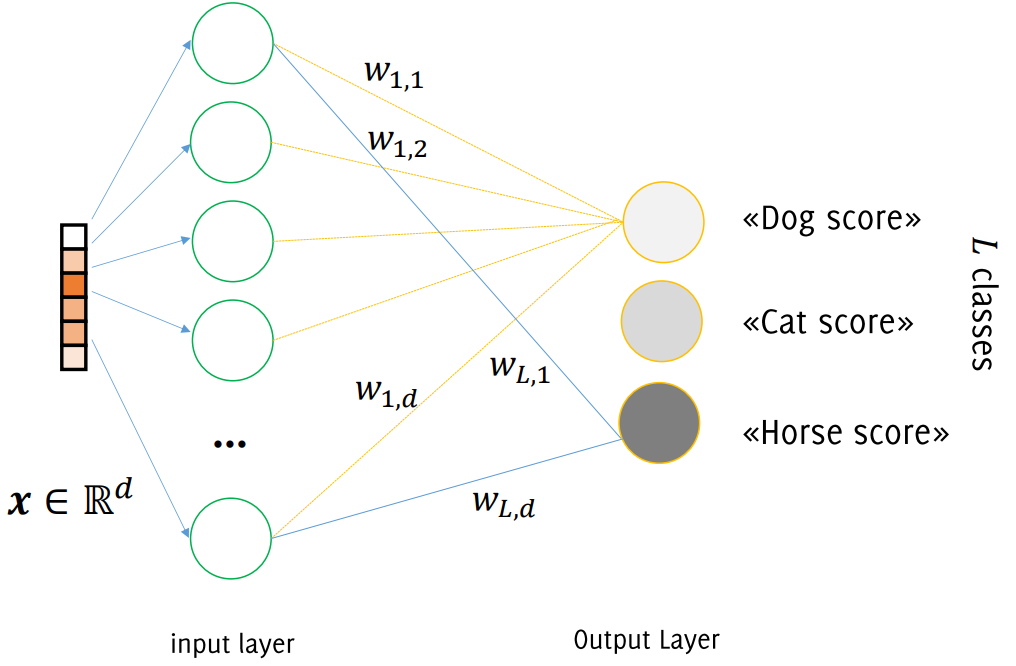
\includegraphics[width=0.75\linewidth]{images/nn.png}
    \caption{Neural Network for CIFAR-10 dataset}
\end{figure}
The classifier's weights can be organized in a matrix$\mathbf{W}\in\mathbb{R}^{L\times d}$, where $L$ is the number of classes and $d$ is the image's flattened dimension.
The score for the $i$-th class is computed as the inner product of the image vector $\mathbf{x}$ and the corresponding row in $\mathbf{W}$: 
\[s_i=\mathbf{W}[i,:]\mathbf{x}+b_i\]
Since this is a single-layer network, nonlinearity is not necessary, and the softmax activation can be omitted, as it does not affect the ranking of class scores.

\subsection{Linear classifier for images}
An image classifier can be understood as a function that maps an image $\mathbf{I}$ to a confidence score vector $\mathcal{K}(\mathbf{I})\in\mathbb{R}^L$, where the $i$-th component $s_i$ represents the score indicating the likelihood that the image belongs to class $i$.
A good classifier assigns the correct class to the highest score.
In the case of linear classification, $\mathcal{K}$ is a linear function mapping the image vector $\mathbf{x}\in\mathbb{R}^d$ to class scores:
\[\mathcal{K}(\mathbf{x})=\mathbf{Wx}+b\]
Here, $\mathbf{W}\in\mathbb{R}^{L\times d}$ is the weight matrix, and $b\in\mathbb{R}^L$ is the bias vector. 
The predicted label for an input image is the class with the highest score:
\[\hat{y}_j=\argmax_{i=1,\dots,L}[\mathbf{s}_j]_\mathbf{i}\]
Here, $[\mathbf{s}_j]_\mathbf{i}$ is the $i$-th component of the score vector $\mathbf{s}=\mathbf{Wx}+\mathbf{b}$
The score for each class is the weighted sum of pixel values, with the weights being the learned parameters of the classifier.

\subsection{Linear classifier training}
The goal of training is to find the parameters $\mathbf{W}$ and $\mathbf{b}$ that minimize the overall loss on the training set.
For a linear classifier, this can be formulated as:
\[[\mathbf{W},\mathbf{b}]=\argmin_{\mathbf{W}\in\mathbb{R}^{L\times d},\mathbf{b}\in\mathbb{R}^L}\sum_{(\mathbf{x}_i,\mathbf{y}_i)\in\text{training set}}\mathcal{L}_{\mathbf{W},\mathbf{b}}(\mathbf{x},y_i)\]
Here, $\mathcal{L}_{\mathbf{W},\mathbf{b}}$ is the loss function that quantifies the error between the predicted and true labels.

\paragraph*{Loss function}
The loss function $\mathcal{L}$ measures how well the classifier performs on the training images, assigning high values to misclassified examples and low values to correct ones.
It is typically minimized using gradient descent and its variants. 
Regularization is often applied to the loss function to avoid overfitting, ensuring a well-behaved solution:
\[[\mathbf{W},\mathbf{b}]=\argmin_{\mathbf{W}\in\mathbb{R}^{L\times d},\mathbf{b}\in\mathbb{R}^L}\sum_{(\mathbf{x}_i,\mathbf{y}_i)\in\text{training set}}\mathcal{L}_{\mathbf{W},\mathbf{b}}(\mathbf{x},y_i)+\lambda\mathcal{R}(\mathbf{W},\mathbf{b})\]
Here, $\lambda>0$ is a regularization parameter that controls the trade-off between fitting the training data and maintaining model simplicity.

\paragraph*{Geometric interpretation}
Each image is represented as a point in $\mathbb{R}^d$, and the classifier corresponds to a linear function in this space. 
In the 2D case, this function would be:
\[f([x_1,x_2])=w_1x_1+w_2x_2+b\]
The decision boundary where $f([x_1,x_2])=0$ is a line, separating positive and negative class scores.
In higher dimensions, this decision boundary generalizes to a hyperplane in $\mathbb{R}^d$. 

\subsection{Image classification challenges}
The main challenges in image classification are: 
\begin{enumerate}
    \item \textit{Dimensionality}: images and videos are high-dimensional data, making it challenging to manage memory and computational resources. 
        Entire batches of images and their activations must be stored during training.
    \item \textit{Label ambiguity}: a single label may not fully capture the content of an image, making the classification task inherently ambiguous.
    \item \textit{Invariance to transformations}: many transformations, such as changes in illumination, deformations, or viewpoint, can alter an image significantly while preserving its label. 
        Robust classifiers must account for these variations.
    \item \textit{Inter-class variability}: images within the same class may differ significantly, making it hard to find common patterns for classification.
    \item \textit{Perceptual similarity}: similarity between images does not always correspond to pixel-level similarity. 
        For instance, assigning the closest training image's label to a test image using nearest-neighbor methods like $k$-NN can be problematic in high-dimensional spaces.
\end{enumerate}
In $k$-nearest neighbors ($k$-NN), the class of a test image is predicted by the most frequent label among its $k$-closest images in the training set:
\[\hat{y}_j=\argmax_{i=1,\dots,L}y_{j^\ast}\]
Here, $j^\ast$ represents the mode of the $k$-nearest images, and the distance function $d(\cdot)$ could be Euclidean or Manhattan distance.
Setting the parameters $k$ and the distance measure is an issue. 
Although $k$-NN is easy to implement and requires no training, it is computationally expensive at test time and struggles with high-dimensional data like images.

\subsection{Feature extraction}

Images cannot be directly fed into a classifier, as raw pixel data is often too complex and high-dimensional to yield meaningful results. 
Therefore, an intermediate step is required to extract relevant information and reduce the dimensionality of the data, making it easier for the classifier to work effectively.

Effective feature extraction plays a crucial role: the quality of the features directly impacts the performance of the classifier. 
The goal is to capture the most important aspects of the image while minimizing irrelevant information.

\paragraph*{Handcrafted features}
The advantages of handcraft features are: 
\begin{itemize}
    \item \textit{Leverage prior domain expertise}: features are often designed by experts who understand the problem and the data.
    \item \textit{Interpretability}: handcrafted features tend to be easier to understand, which helps in diagnosing why certain features work or fail.
    \item \textit{Tunability}: features can be adjusted and fine-tuned based on performance feedback, allowing for more control over the classification process.
    \item \textit{Efficient with limited data}: handcrafted features often require less data to train compared to deep learning methods.
    \item \textit{Feature weighting}: it is possible to give more importance to certain features that are known to be relevant to the task at hand.
\end{itemize}
While the drawbacks are: 
\begin{itemize}
    \item \textit{Labor-intensive}: designing and programming handcrafted features requires significant time and effort.
    \item \textit{Limited applicability}: in many visual recognition tasks, handcrafted features are less effective than automated feature extraction methods, as human-designed features may miss important patterns.
    \item \textit{Risk of overfitting}: since the features are tailored to a specific training set, there is a risk of overfitting, which leads to poor generalization on new data.
    \item \textit{Lack of generalization}: handcrafted features are often problem-specific and may not transfer well to other tasks or datasets.
\end{itemize}

Rather than relying on handcrafted features, which require manual design and domain expertise, we can leverage data-driven features. 
These features are automatically learned from the data itself, offering a more scalable and effective approach. 
This is achieved by using a Convolutional Neural Network, which is specifically designed to extract hierarchical features from images.

CNNs learn to identify patterns such as edges, textures, and more complex structures through multiple layers of convolution and pooling, allowing them to capture increasingly abstract representations of the image. 
This eliminates the need for manual feature engineering and often results in superior performance, particularly in tasks like image classification, object detection, and visual recognition. 
By letting the model discover the most relevant features directly from the data, CNNs reduce human bias and can generalize better to new, unseen data.